\documentclass[a4paper, english]{scrartcl}

\usepackage[english]{babel}
\usepackage{tabularx}
\usepackage{graphicx}
\usepackage{booktabs}
\usepackage{microtype}
% TODO Fix title below
\usepackage[pdftitle = {TODO TITLE HERE}, colorlinks = true, urlcolor = blue, linkcolor = blue, citecolor = blue]{hyperref}

% TODO Fix title here
\title{Optical Character Recognition}
\subtitle{Subtitle here \ldots}
% TODO Add names here
\author{Irvin,~Duane \\ \texttt{duane@student.chalmers.se}
  \and Karlsson,~Pontus \\ \texttt{ponkarls@student.chalmers.se}
  \and Holm,~Jesper \\ \texttt{~holmje@student.chalmers.se}
  \and Subramanian,~Aditya \\ \texttt{email@student.chalmers.se}
}
\date{DATE HERE, 2017}

\begin{document}

\clearpage\maketitle
\thispagestyle{empty}

\pagebreak

\setcounter{page}{1}
\hypersetup{linkcolor=black}
\tableofcontents

\pagebreak

\section{Introduction}
\subsection{Background}
This project being performed on behalf of Cybercom,
a Nordic IT consulting company with multiple offices throughout the world.
This project will be done in cooperation with the Cybercom Gothenburg office.
The purpose of the project is to design a system capable of recognizing text 
in an image and convert it into text or audio output. 
The primary project description is kept as simple as possible. 
However the intention is that if the primary functionality and tests are 
finished the project scope and functionality can be extended depending on 
time and resource constraints. 
In the future the project could be expanded into a hardware implementation 
to be used by vision impaired people with text to speech functionality.
\subsection{Purpose}
The primary purpose of this project is to create a character recognition
system using pre-existing libraries such as OpenCV. 
A secondary purpose is for Cybercom to build a connection with students 
who may become future engineers. 
\subsection{Vision}
The goal of this project is to develop a software that can recognise 
characters on a image file. 
The image is suppose to be taken with a laptop camera or something equivalent.
And the software should be running on an Linux or Android platform. 
For starters we are going to aim at single character recognition.
Once the character is recognised it should be printed to a text file.
If there is time, there will be further development on word recognition and
to translate words to voice.

Features below are denoted with RF for required features and OF for optional
features.
  \noindent\begin{tabularx}{\linewidth}{X p{0.75\linewidth}}
  \toprule
    \textbf{Feature} & \textbf{Description} \\
  \midrule
  RF-1 &
    From an image, recognize characters with an accuracy of at least 60\%.
    Preferably better than 80\%.\\
  RF-2 &
    Turn text into English speech output. \\
  RF-3 &
    User interface that implements RF-1 and RF-2. \\
  OF-1 &
    Add functionality and improve performance to make the product compatible
    with mobile devices. \textit{TBD} \\
  OF-2 &
    Use dictionary for correction of recognized words. \textit{TBD} \\
  \bottomrule
  \end{tabularx}
\subsection{Scope}

\section{Method}
\textit{TBD}

\subsection{Testing}
\textit{TBD}

\section{Technical Background}
\textit{TBD}

\section{Implementation}
Due to time and resource considerations, the scope of the project was decreased.
Naturally, this had impact on the overall system architecture and requirements.
The current scope of the project is outlined in detail below.

Instead of a video feed, which was the original intention, the input to the
system will be static images either saved on a hard drive or in memory. Going
from a video feed to static images also removes the need for implementation of
any motion and/or image tracking. The requirement for the detection/error rate
was altered from 90\% to 60\% which is expected by Tesseract.

The output is going to be a text file although an implementation of
Text-To-Speech (TTS) is realistic and will be considered at a later stage of
the project.

To summarize, the system will take in a static image as an input, run
character recognition and output the result. The output is text-based but
Text-to-Speech (TTS) may be implemented in the final product.
\subsection{Use cases}
\textit{TBD}

\subsection{UML/Modules}
\textit{TBD}
\begin{figure}[h!]
  \centering
  % TODO Fix label
  \caption{\textit{TBD}}\label{fig:ex1a}
  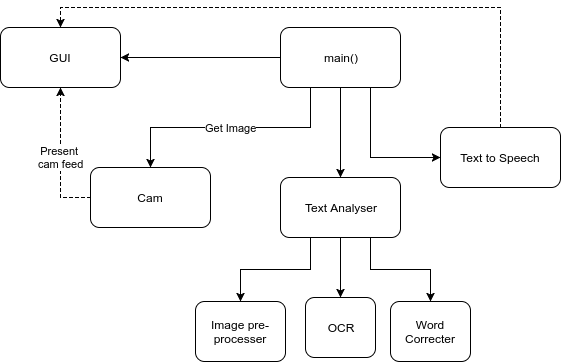
\includegraphics[width=1.0\textwidth]{res/UML1}
\end{figure}

\subsection{Tests}
\textit{TBD}

\section{Result}
\textit{TBD}

\section{Discussion}
\textit{TBD}

\pagebreak
% Ask me how to properly insert references // Duane
\bibliography{references}
\bibliographystyle{ieeetr}

\end{document}
